\documentclass[12pt]{article}
\renewcommand{\baselinestretch}{1}
\usepackage{graphicx}
\usepackage{subcaption}
\usepackage{wrapfig}
\usepackage{multicol}
\usepackage{lipsum}
\usepackage{microtype}
\usepackage{vwcol}

%\usepackage{subfig}
\usepackage{float}
\usepackage[nottoc, notlot, notlof]{tocbibind}
\usepackage[margin = 1in]{geometry}
\usepackage{titlesec}
\usepackage{amsfonts, amsmath, amssymb}
\usepackage{hyperref}
\usepackage{tikz}
\usetikzlibrary{shapes.geometric, arrows}
\titleformat*{\section}{\LARGE\bfseries}
\titleformat*{\subsection}{\Large\bfseries}
\titleformat*{\subsubsection}{\Large\bfseries}
%\newcommand{\sectionbreak}{\clearpage}


\tikzstyle{process1} = [rectangle, rounded corners, minimum width=3cm, minimum height=1cm, text centered, draw=black, fill=orange!30]
\tikzstyle{process2} = [rectangle, rounded corners, minimum width=3cm, minimum height=1cm, text centered, draw=black, fill=pink!30]
\tikzstyle{decision} = [diamond, minimum width=3cm, minimum height=1cm, text centered, draw=black, fill=green!30]
\tikzstyle{arrow} = [thick,->,>=stealth]


\begin{document}

\begin{titlepage}
 
\begin{minipage}[c]{0.2\linewidth}

\includegraphics[width=1.0\textwidth]{iiserb_logo.png}
\end{minipage} % no space if you would like to put them side by side
\begin{minipage}[c]{0.8\linewidth}
\begin{center}
\begin{Large}
\textbf{Indian Institute of Science Education and \\ \vspace*{-1mm}Research Bhopal}\\ \vspace*{-1mm}
Department of Chemistry\\ \vspace{1mm}
\large{\textit{9$^{th}$ Semester BS-MS project progress report, December 2020}}
\end{Large}
\end{center}
\end{minipage}  
\vspace{3mm}
\begin{center}
\begin{Large}
\textbf{Development and testing of a python based Trajectory-Surface-Hopping code for simulating Non-adiabatic chemical phenomena}
\end{Large}
\end{center}
\vspace{3mm}

\begin{tabbing} % Enables tabbing
\hspace{8cm} \= \hspace{4cm} \= \kill 
{\bf Report by} \> : \textbf{Md. Elious Ali Mondal}\\ 
{\bf Roll Number } \> : \textbf{16111} \\ 
{\bf Supervisor} \> : \textbf{Dr. Varadharajan Srinivasan (Chemistry)} \\
\end{tabbing}
\vspace{2mm}
\begin{tabbing}
\hspace{8cm} \= \hspace{4cm} \= \kill
{\bf Review Committee members} \> : \textbf{Dr. Rati Sharma (Chemistry)}\\
{} \> : \textbf{Dr. Y. Adithya Lakshmanna (Chemistry)}
\end{tabbing}
\vspace{20mm}
\begin{center}
\large\textbf{Declaration}\\
\end{center}
\begin{large}
I, \textbf{Md. Elious Ali Mondal}, hereby confirm that the text written here is my own
work and is not copied from other person’s work (published or unpublished).\\

\vspace{10mm}
Md. Elious Ali Mondal \hspace{3.85cm} Bhopal \hspace{2.5cm} 06/12/20 \\  \textbf{Students Digital Signature} \hspace{3cm} \textbf{Place} \hspace{3cm} \textbf{Date}
\end{large}

\end{titlepage}


\tableofcontents
\thispagestyle{empty}
\clearpage
%\listoffigures
%\listoftables
\setcounter{page}{1}

\section{Abstract}
The excited state of many molecules have crossings between their potential energy surface giving rise to non-adiabaticity. Due to this, we can't treat these states under the Born-Oppenheimer approximation(BOA). To go beyond the BOA, we have to either do the full quantum treatment of the system (i.e. the nuclei are also treated quantum mechanically, which is computationally very expensive) or resort to some other semi-classical approach which can account for the non-adiabaticity. One such approach, suggested by John Tully\cite{tully} called Fewest-Switches-Surface-Hopping(FSSH) has been able to successfully model the non-adiabatic effects in lots of molecules like photo-relaxation of nucleo-bases, photo-isomerizarion of azo-benzenes. We are developing a python based Trajectory-Surface-Hopping code as a wrapper for an already existing open-source electronic structure code, NWChem.  

\section{Introduction}
Suppose we have an electron ($e^-$) in the ground state of an infinite well. Now, lets start stretching the well. The stretching can be done in two extrme way:
\begin{enumerate}
\item[\textbf{a}]{If we stretch \textbf{very slowly}, we will find that the $e^-$ still remains in the ground state of the stretched well. This change is said to be  adiabatic.}
\item[\textbf{b}]{If we stretch \textbf{very fast} (sudden stretch), the electronic wavefunction will now be a superposition of the eigenstates of the stretched well. This is called a non-adiabatic change.}
\end{enumerate}
\subsection{Non-adiabaticity in Quantum Mechanics}
In general, if we have our system to be in the $i^{th}$ eigenstate, $\Psi_i$ of the Hamiltonian $\hat{H}$. 	Then, with time, the system evolves according to Schr\"{o}dinger equation as:
\begin{equation}\label{eq:1}
i\hbar\frac{\partial \Psi_i}{\partial t} = \hat{H}\Psi_i
\end{equation}
If we assume that we can form instantaneous eigenvalues of the time-dependent hamiltonian, then,
\begin{equation}\label{eq:2}
\hat{H}(t)\phi_j(t) = E(t)\phi_j(t) \hspace{1cm} \text{and} \hspace{1cm} \Psi_i(t) = \sum_i c_j(t)\phi_j(t)
\end{equation}
Putting eqn(\ref{eq:2}) in eqn(\ref{eq:1}) and rearranging a little will give us,
\begin{equation}\label{eq:3}
\underbrace{i\hbar\dot{c}_k(t) = c_k(t)E_k(t)}_\text{adiabatic part} - \underbrace{i\hbar \sum_jc_j\frac{\langle\phi_k|\dot{\hat{H}}|\phi_j\rangle}{E_j-E_k}}_\text{non-adiabatic part}
\end{equation}
In the above equation, the dot represents time derivative of that quantity. So, non-adiabaticity can occur if either the hamiltonian changes very fast or(and) when the instantaneous wavefunctions are nearly degenerate.

\subsection{Born-Oppenheimer Approximation (BOA)}
For molecules, the hamiltonian, in atomic units, can be written as;
\begin{equation}\label{eq:4}
\hat{H}(\textbf{r},\textbf{R}) 
= 
\overbrace{-\sum_A\frac{\nabla_A^2}{2M_A}}^\text{Nuclear Kinetic energy}
-
\underbrace{\sum_i\frac{\nabla_i^2}{2}+\sum_{i,j>i}\frac{1}{|\textbf{r}_i-\textbf{r}_j|} -\sum_{A,i}\frac{1}{|\textbf{R}_A-\textbf{r}_i|}}_\text{Electronic part} 
+
\overbrace{\sum_{A,B>A}\frac{1}{|\textbf{R}_A-\textbf{R}_B|}}^\text{Nucleus-Nucleus repulsion}
\end{equation}
Since $\textbf{M}_{Nu} >> \textbf{m}_{e^-}$, usually we neglect the first term of eqn(\ref{eq:4}) and make the electronic motion independent of the nuclear motion and we solve only for the effective electronic hamiltonian, $\hat{H}_{e^-}$.
\begin{equation}\label{eq:5}
\hat{H}_{e^-}(\textbf{r};\textbf{R})\Psi_{e^-}(\textbf{r};\textbf{R}) = E_{e^-}(\textbf{R})\Psi_{e^-}(\textbf{r};\textbf{R})
\end{equation} 
where
\begin{equation}\label{eq:6}
\hat{H}_{e^-}(\textbf{r};\textbf{R}) = \sum_i\frac{\nabla_i^2}{2}+\sum_{i,j>i}\frac{1}{|\textbf{r}_i-\textbf{r}_j|} -\sum_{A,i}\frac{1}{|\textbf{R}_A-\textbf{r}_i|}
\end{equation}
We are now treating the \textbf{R} as a parameter instead of a variable in eqn(\ref{eq:5}) and eqn(\ref{eq:6}). So, scanning through different nuclear configurations(\textbf{R}) we can form an electronic Potential energy surface(PES) $E_{e^-}(\textbf{R})$.

\subsection{Breakdown of BOA}
The BOA is a type of adiabatic approximation where we assume that the electronic and nuclear motion decouple as the nuclei move very slow compared to $e^-$. So effectively, we assume that $\dot{H}$ in the second term of eqn(\ref{eq:3}) is very small and hence the $\Psi_{e^-}$ can evolve independent of the nuclear wavefunction. Due to this, 
$\Psi_{e^-}(\textbf{r};\textbf{R})$ are called adiabatic basis and the $E_{e^-}(\textbf{R})$ are called adiabatic surfaces or adiabats. Ignoring the last term of eqn(\ref{eq:3}) will make the nuclei to propagate only along a single PES.
\vspace{2mm}

The BOA has made it possible to describe the ground-state properties of a lot of molecules. But some molecules, when excited, show crossings or near-degeneracy of different excited states i.e. the non-adiabatic term of eqn(\ref{eq:3}) blows up, which gives rise to many non-adiabatic phenomena and we can no longer treat those systems under BOA.
\vspace{2mm}

In regions of strong coupling between the excited state PES, the actual wavepacket should branch off. To capture the branching off of nuclear wavepackets, Tully,in 1990\cite{tully},  gave a method known as Fewest-Switches-Surface-Hopping(FSSH). In this method, we simulate an ensemble of trajectories, each starting with different(or same) initial conditions, allowing the nuclei to evolve on a single adiabatic PES but with a possibility to hop to different PES in regions of strong coupling, based on a stochastic algorithm. It is assumed that when we take average of the populations from all the independent trajectories we will be account for the non-adiabaticity of the system.

\section{Methods}
\subsection{Fewest Switches Surface Hopping - Theory}
%\begin{small}
We consider our electronic wavefunction to be superposition of different electronic states $\Phi_k$, 
\begin{equation}\label{eq:7}
\Psi(\textbf{r};\textbf{R}(t)) = \sum_kc_k(t)\Phi_k(\textbf{r};\textbf{R}(t)) 
\end{equation}
Now we propagate the nuclei for a trajectory by Newton's equation of motion,
\begin{equation}\label{eq:8}
M_I\ddot{\textbf{R}} = -\nabla E_k(\textbf{R}(t))
\end{equation}
where \textbf{R} are the nuclear coordinates and $E_k(\textbf{R})$ is the PES corresponding to $\Phi_k(\textbf{r};\textbf{R})$. The electronic coefficients evolve by eqn(\ref{eq:3}), which in density matix notation is,
\begin{equation}\label{eq:9}
i\hbar\dot{\rho}_{kj} = \rho_{kj}(E_k(\textbf{R})-E_j(\textbf{R})) - i\hbar \sum_l\left\lbrace\rho_{lj}\textbf{d}_{kl}\textbf{.}\dot{\textbf{R}} + \rho_{kl}\textbf{d}_{lj}\textbf{.}\dot{\textbf{R}}\right\rbrace
\end{equation}
where
\begin{equation}\label{eq:10}
\textbf{d}_{mn} = \frac{\langle\Phi_m|\nabla_\textbf{R}\hat{H}|\Phi_n\rangle}{E_n-E_m} = \langle\Phi_m|\nabla_\textbf{R}|\Phi_n\rangle
\end{equation}
The $\textbf{d}_{mn}$ are the measure of coupling between different PES and are also termed as Non-adiabatic couplic vectors(NACV) and the combined $\textbf{d}_{mn}\textbf{.}\dot{\textbf{R}}$ term is called Non-adiabatic couplings (NAC) and is sometimes denoted by $\sigma_{mn}$. The diagonal terms of this matrix are called populations and they evolve as,
\begin{equation}\label{eq:11}
\dot{\rho}_{kk} = -\sum_{l \neq k}2\text{Re}(\rho_{kl}^*\textbf{d}_{kl}\textbf{.}\dot{\textbf{R}}) = \sum_{l\neq k}\gamma_{kl}
\end{equation}
Due to the couplings between the different surfaces, there is chance that the nuclei may hop from from one surface to another. The probability of a hop $j\rightarrow k$ in between time \textit{t} and $t+dt$ is calculated by,
\begin{equation}\label{eq:12}
\begin{split}
P_{j\rightarrow k}(t) &= \frac{\text{change in population of k due to j}}{\text{population of j}}\\
&= max\left[0,\frac{\gamma_{kj}dt}{\rho_{jj}}\right]
\end{split}
\end{equation} 
The switch from an electronic state \textit{j} to \textit{k} will occur if,
\begin{equation}\label{eq:13}
\sum_{m=1}^{k-1}P_{j\rightarrow m} < \zeta <  \sum_{m=1}^{k}P_{j\rightarrow m}
\end{equation}
where $\zeta$ is a random rumber between 0 and 1.
%\end{small}
 
\subsection{Fewest Switches Surface Hopping - Algorithm}
\vspace{15mm}

\begin{center}
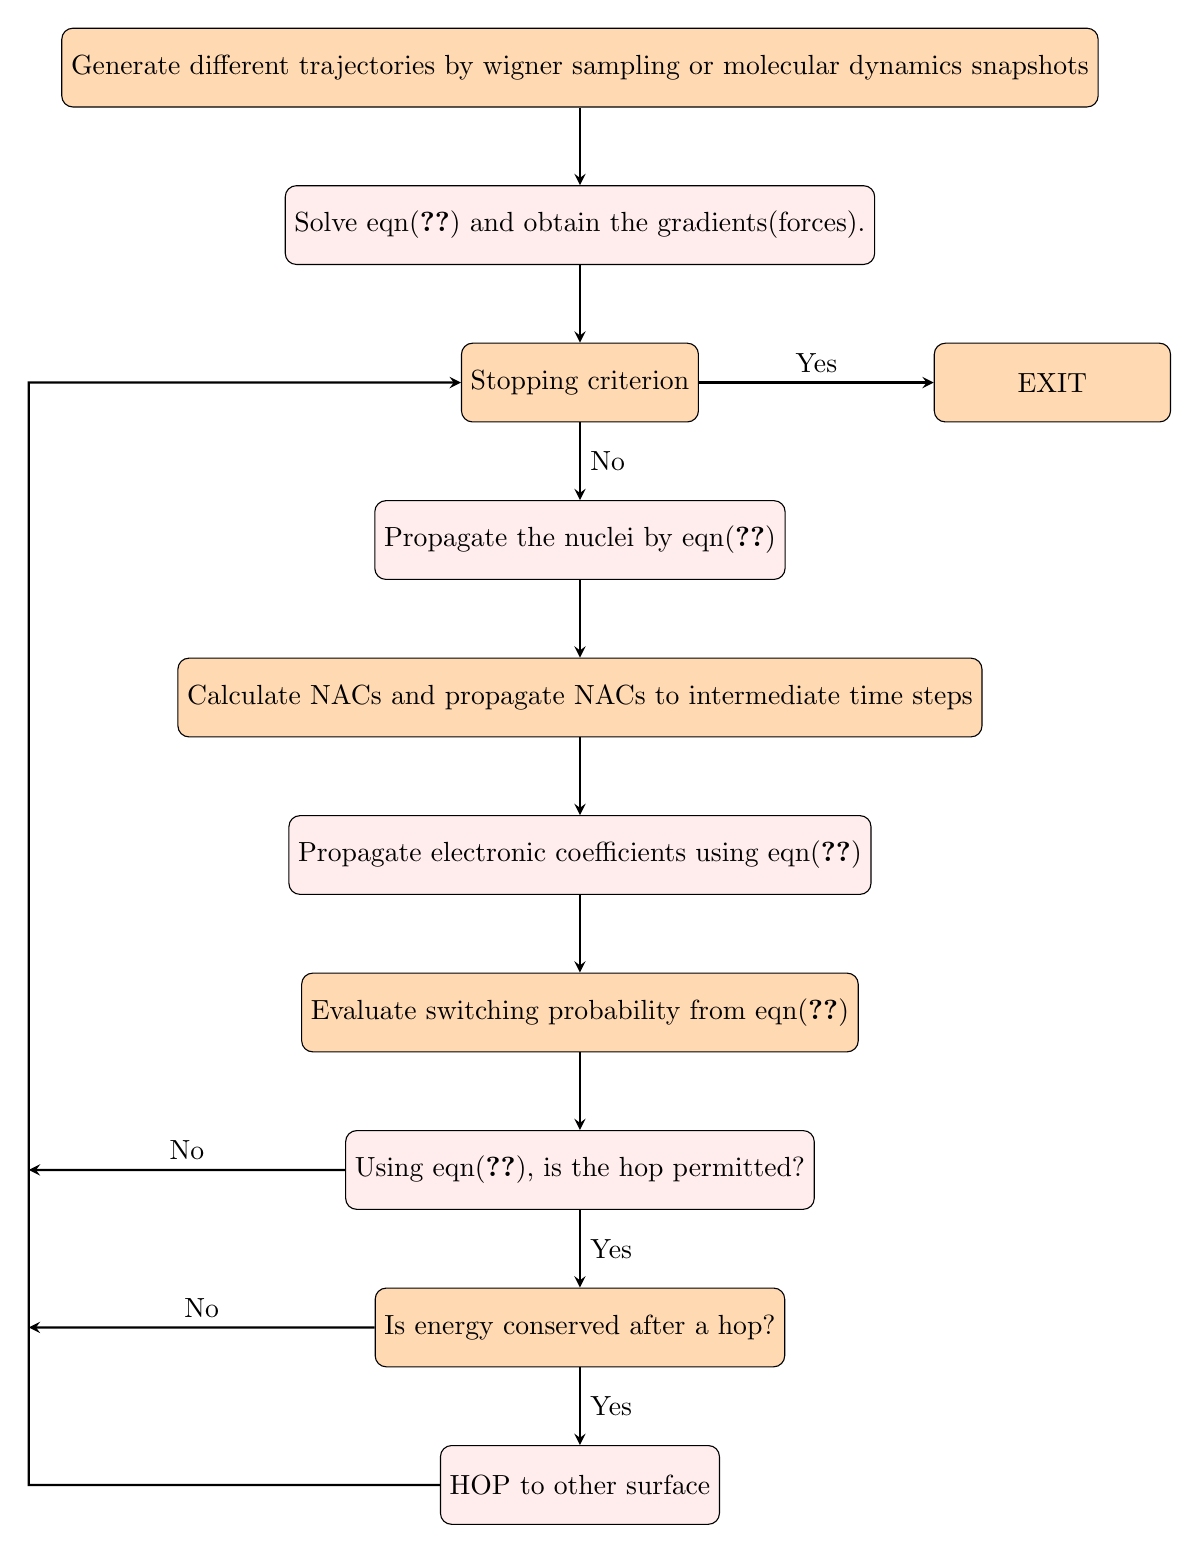
\begin{tikzpicture}[node distance=2cm]
\node (proc1) [process1] {Generate different trajectories by wigner sampling or molecular dynamics snapshots};
\node (proc2) [process2, below of=proc1] {Solve eqn(\ref{eq:5}) and obtain the gradients(forces).};
\node (proc3) [process1, below of=proc2] {Stopping criterion};
\node (proc4) [process1, right of=proc3, xshift=4cm] {EXIT};
\node (proc5) [process2, below of=proc3] {Propagate the nuclei by eqn(\ref{eq:8})};
\node (proc6) [process1, below of=proc5] {Calculate NACs and propagate NACs to intermediate time steps};
\node (proc7) [process2, below of=proc6] {Propagate electronic coefficients using eqn(\ref{eq:3})};
\node (proc8) [process1, below of=proc7] {Evaluate switching probability from eqn(\ref{eq:12})};
\node (proc9) [process2, below of=proc8] {Using eqn(\ref{eq:13}), is the hop permitted?};
\node (proc10) [process1, below of=proc9] {Is energy conserved after a hop?};
\node (proc11) [process2, below of=proc10] {HOP to other surface};

\draw [arrow] (proc1) -- (proc2);
\draw [arrow] (proc2) -- (proc3);
\draw [arrow] (proc3) -- node[anchor=south] {Yes} (proc4);
\draw [arrow] (proc3) -- node[anchor=west] {No} (proc5);
\draw [arrow] (proc5) -- (proc6);
\draw [arrow] (proc6) -- (proc7);
\draw [arrow] (proc7) -- (proc8);
\draw [arrow] (proc8) -- (proc9);
\draw [arrow] (proc9) -- node[anchor=west] {Yes} (proc10);
\draw [arrow] (proc9) -- node[anchor=south] {No} (-7,-14);
\draw [arrow] (proc10) -- node[anchor=west] {Yes} (proc11);
\draw [arrow] (proc10) -- node[anchor=south] {No} (-7,-16);
\draw [arrow] (proc11) -- (-7,-18) -- (-7,-4) -- (proc3);


\end{tikzpicture}
\end{center}

\subsection{Decoherence Corrections to FSSH}
Tully's FSSH algorithm has an internal problem of overcoherence. Consider the Born-Huang ansatz for total wavefunction of the combined nuclei-electron system:
	\begin{equation}\label{eq:14}
	|\Psi\rangle = \sum_i f_i|\chi_i\rangle|\phi_i\rangle 
	\end{equation}
where the $\chi$ and $\phi$ are nuclear and electronic wavefunctions respectively. From here, we can find the electronic density matrix to be
\begin{equation}\label{eq:15}
	\sigma_{el} = \sum_{i,j} f_j^*f_i\langle\chi_j|\chi_i\rangle|\phi_i\rangle\langle\phi_j|
	\end{equation}
From eqn(\ref{eq:7}), we can find the density matrix in FSSH as,
\begin{equation}\label{eq:16}
\sigma_{el} = \sum_{i,j} c_ic_j^*|\phi_i\rangle\langle\phi_j|
\end{equation}
Comparing eqns (\ref{eq:15}) and (\ref{eq:16}), we can see that 
\begin{equation}\label{eq:17}
 c_ic_j^* = f_j^*f_i\langle\chi_j|\chi_i\rangle 
\end{equation}
So, after passing the strong-nuclear coupling region, when the branched off-nuclear wavepackets' overlap i.e. $\langle\chi_j|\chi_i\rangle\rightarrow 0$ and so the $c_ic_j^*$ should also vanish. But, there is no such term in the FSSH equations which can do so and so the problem of overcoherence arises. To deal with this, some decoherence corrections have been suggested\cite{decoherence}:
\begin{enumerate}
\item{\textbf{Instantaneous Decoherence correction Simple(IDC-S) :} After each successful hop, the electronic wavefunction is reinitialised as a pure state in the current electronic state.}
\item{\textbf{Instantaneous Decoherence correction Accepted (IDC-A) :} If a hop is accepted, the wavefunction is made to collapse at the current state and if a hop is forbidden, the wavefunction is collapsed back to the current running state.}
\item{\textbf{Energy Based Decoherence Correction (EDC) :} Instead of instantaneous collapse, here we allow for decay of the electronic wavefunction to a particular state. If the current PES is of $\alpha$ and $\beta$ represents other electronic states, then, 
    \begin{equation}\label{eq:18}
	c_\beta'(t) = c_\beta(t)e^{\frac{-\Delta t}{\tau_{\beta\alpha}(t)}}
    \end{equation}
    and the loss gets accumulated in the current state as:
    \begin{equation}\label{eq:19}
    c_\alpha'(t) = c_\alpha(t)\left[\frac{1-\sum_{\beta\neq\alpha}|c_\beta'(t)|^2}{|c_\alpha'(t)|^2}\right]^{\frac{1}{2}}
    \end{equation}    	 
    $\tau_{\beta\alpha}$ is known as the decoherence time and Granucci \textit{et al.}\cite{granucci} suggested it to be:
    \begin{equation}\label{eq:20}
    \tau_{\beta\alpha}(t) = \frac{\hbar}{|E_\beta(t)-E_\alpha(t)|}\left(C+\frac{E_0}{E_{kin}}\right)
    \end{equation}}
\end{enumerate}

\section{Results}
An in-house python-code for simulating the FSSH has been already written and it is in the testing phase. For caclulating the PES and getting the auxiliary excited state wavefunctions we are using LR-TDDFT formalism. The test for testing the correctness of NAC algorithm has been done on Ethylene molecule with 6-31G* basis set and B3LYP as the density functional.\\
 
\begin{figure}[h]
\begin{subfigure}{.5\textwidth}
  \centering
  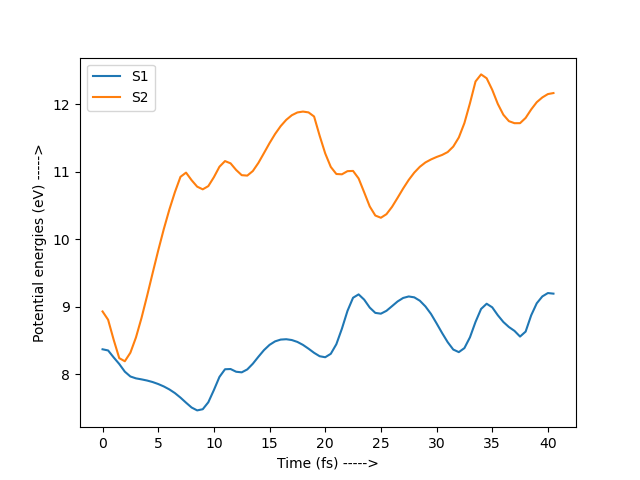
\includegraphics[width=1.0\linewidth]{PES_23.png}
  \caption{PES}
  \label{fig:sfig1}
\end{subfigure}%
\begin{subfigure}{.5\textwidth}
  \centering
  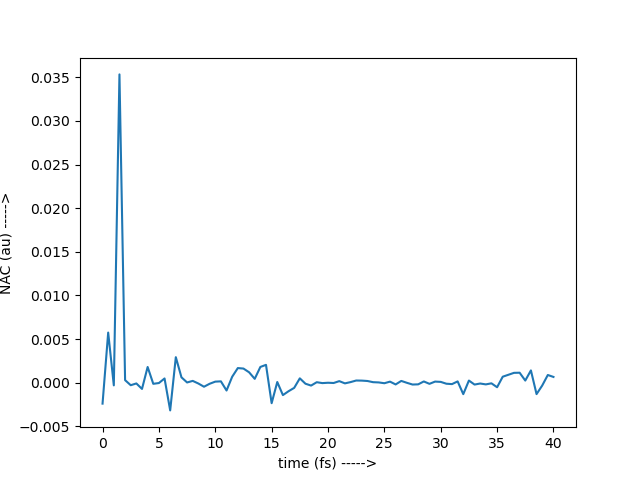
\includegraphics[width=1.0\linewidth]{nac_23.png}
  \caption{NAC}
  \label{fig:sfig2}
\end{subfigure}
\caption{PES and NAC between $1^{st}$(S1) and $2^{nd}$(S2) excited states}
\label{fig:NAC_23}
\end{figure}
\begin{figure}[h]
\begin{subfigure}{.5\textwidth}
  \centering
  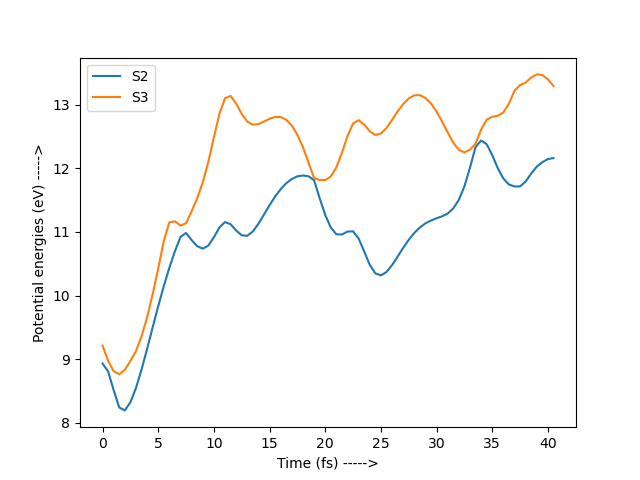
\includegraphics[width=1.0\linewidth]{PES_34.png}
  \caption{PES}
  \label{fig:sfig1}
\end{subfigure}%
\begin{subfigure}{.5\textwidth}
  \centering
  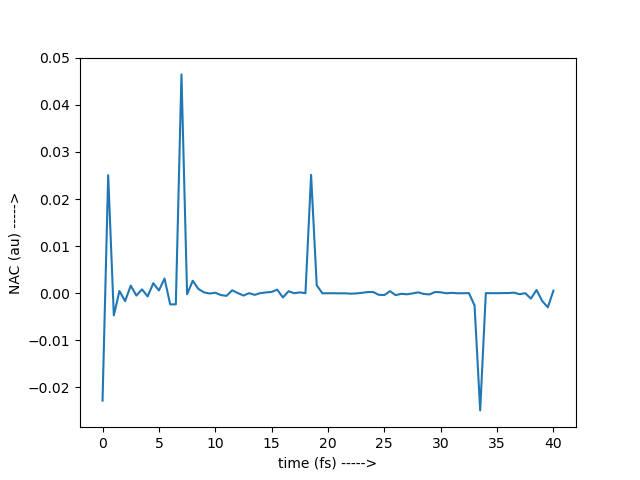
\includegraphics[width=1.0\linewidth]{nac_34.png}
  \caption{NAC}
  \label{fig:sfig2}
\end{subfigure}
\caption{PES and NAC between $2^{nd}$(S2) and $3^{rd}$(S3) excited states}
\label{fig:NAC_23}
\end{figure}
From the above figures, we can see that at the time steps where the PES are very close in energy, the NAC shoots up indicating that our implementation of NAC in the code is correct. We need to do more simulations and further compare with established results for verifying the qualitative correctness of our code.

\section{Discussion and future plans}
We have tested the NAC part of the and are now testing for the electronic propagation part. After this is tested and benchmarked with some already reported results\cite{werner,curchod}, we will test for the decoherence corrections in FSSH, for which the code is already written. We further aim to add more functionalities to the code like calculations of NAC-vectors and if time permits, we will also try to work on QM/MM implementation. 


\begin{thebibliography}{9}
\bibitem{tully} 
John C. Tully, "Molecular dynamics with electronic transitions"
\textit{\href{http://dx.doi.org/10.1039/A801824C}{The Journal
of Chemical Physics 93.2 (1990), pp. 1061–1071}}. 

\bibitem{decoherence} 
T. Nelson, S. Fernandez-Alberti, A. E. Roitberg, and S. Tretiak "Nonadiabatic excited-state molecular dynamics: Treatment of electronic decoherence"
\textit{\href{https://doi.org/10.1063/1.4809568}{J. Chem. Phys. 138, 224111 (2013)}}.

\bibitem{granucci} 
Granucci \textit{et. al. }"Including quantum decoherence in surface hopping"
\textit{\href{https://doi.org/10.1063/1.3489004}{The Journal of Chemical Physics 133, 134111 (2010)}}.

\bibitem{werner} 
Werner et al., “Nonadiabatic dynamics within the time dependent density functional theory: Ultrafast photodynamics in pyrazine"  
\textit{\href{https://doi.org/https://doi.org/10.1016/j.chemphys.2008.02.061}{Chemical Physics 349.1 (2008)}}.

\bibitem{curchod} 
L.M.Ibele and B.F.E.Curchod "A molecular perspective on Tully models for nonadiabatic dynamics"
\textit{\href{https://doi.org/10.1039/D0CP01353F}{Phys. Chem. Chem. Phys, 2020, 22, 15183}}.


\end{thebibliography}
\end{document}
